%%%%%%%%%%%%%%%%%%%%%%%%%%%%%%%%%%%%%%%%%%%%%%%%%%%%%%%%%%%%%%%%%%%%%%%%%%%%%%%%
% preamble
%%%%%%%%%%%%%%%%%%%%%%%%%%%%%%%%%%%%%%%%%%%%%%%%%%%%%%%%%%%%%%%%%%%%%%%%%%%%%%%%

\documentclass{sty/proposal}
\usepackage{textcomp, gensymb, pifont}
\usepackage{url}
\usepackage{tikz}
\usepackage{setspace}
\usepackage{wrapfig}
\usepackage{hyperref}
\usepackage{xspace}
% custom
\usepackage{listings}
\usepackage{color}

\definecolor{dkgreen}{rgb}{0,0.6,0}
\definecolor{gray}{rgb}{0.5,0.5,0.5}
\definecolor{mauve}{rgb}{0.58,0,0.82}

\lstset{frame=tb,
  language=Python,
  aboveskip=3mm,
  belowskip=3mm,
  showstringspaces=false,
  columns=flexible,
  basicstyle={\small\ttfamily},
  numbers=none,
  numberstyle=\tiny\color{gray},
  keywordstyle=\color{blue},
  commentstyle=\color{dkgreen},
  stringstyle=\color{mauve},
  breaklines=true,
  breakatwhitespace=true,
  tabsize=3
}

\renewcommand{\a}{{\hel A}\xspace}
\renewcommand{\b}{{\hel B}\xspace}
\renewcommand{\c}{{\hel C}\xspace}

\newcommand{\cmda}{{\tt ACT}\xspace}
\newcommand{\cmdr}{{\tt READ}\xspace}
\newcommand{\cmdw}{{\tt WRITE}\xspace}
\newcommand{\cmdp}{{\tt PRE}\xspace}
\newcommand{\cmdf}{{\tt REF}\xspace}

\newcommand{\ra}{$\rightarrow$\xspace}
\newcommand{\la}{$\leftarrow$\xspace}

\newcommand{\reqx}{$\mathit{req}_\mathtt{X}$}
\newcommand{\reqy}{$\mathit{req}_\mathtt{Y}$}
\newcommand{\actx}{$\mathtt{ACT}_\mathtt{X}$}
\newcommand{\acty}{$\mathtt{ACT}_\mathtt{Y}$}
\newcommand{\rdx}{$\mathtt{READ}_\mathtt{X}$}
\newcommand{\rdy}{$\mathtt{READ}_\mathtt{Y}$}
\newcommand{\prex}{$\mathtt{PRE}_\mathtt{X}$}
\newcommand{\prey}{$\mathtt{PRE}_\mathtt{Y}$}

\newcommand{\module}[3]{{{\hel #1}$_{\mathrm{#2}}^{\mathrm{#3}}$}\xspace}
\newcommand{\moduledate}[3]{{{\hel #1}$_{\mathrm{#2}}^{\mathrm{#3}}$}\xspace}


\newcommand{\ignore}[1]{}   %comment command for Onur
\newcommand{\checkit}[1]{\textcolor{red}{\textbf{#1}}}

\newcommand\numone{{\large \ding{192}}\xspace}
\newcommand\numtwo{{\large \ding{193}}\xspace}
\newcommand\numthree{{\large \ding{194}}\xspace}
\newcommand\numfour{{\large \ding{195}}\xspace}
\newcommand\numfive{{\large \ding{196}}\xspace}

\newcommand{\trefi}{$t_{\mathit{REFI}}$\xspace}
\newcommand{\trc}{$t_{\mathit{RC}}$\xspace}
\newcommand\trcd{$t_{\mathit{RCD}}$\xspace}
\newcommand\tcl{$t_{\mathit{CL}}$\xspace}
\newcommand\tcwl{$t_{\mathit{CWL}}$\xspace}
\newcommand\tbl{$t_{\mathit{BL}}$\xspace}
\newcommand\tras{$t_{\mathit{RAS}}$\xspace}
\newcommand\trp{$t_{\mathit{RP}}$\xspace}

\newcommand\vdd{$V_{\mathit{DD}}$\xspace}

\newcommand\trcdfar{$t_{\mathit{RCDfar}}$\xspace}
\newcommand\trcfar{$t_{\mathit{RCfar}}$\xspace}
\newcommand\trcdnear{$t_{\mathit{RCDnear}}$\xspace}
\newcommand\trcnear{$t_{\mathit{RCnear}}$\xspace}
\newcommand\trasnear{$t_{\mathit{RASnear}}$\xspace}
\newcommand\trasfar{$t_{\mathit{RASfar}}$\xspace}
\newcommand\trpnear{$t_{\mathit{RPnear}}$\xspace}
\newcommand\trpfar{$t_{\mathit{RPfar}}$\xspace}

\newcommand\cmdact{ACTIVATE\xspace}
\newcommand\cmdpre{PRECHARGE\xspace}
\newcommand\cmdrd{READ\xspace}
\newcommand\cmdwr{WRITE\xspace}

\newcommand{\msc}{SC\xspace}
\newcommand{\mtac}{WMC\xspace}
\newcommand{\mbbc}{BBC\xspace}
\newcommand{\trccritical}{\trc-\emph{critical}\xspace}



\let\oldcelsius\celsius
\renewcommand{\celsius}{~\oldcelsius\xspace}

\newcommand{\DIMMs}[0]{82\xspace}




\newcommand{\titleShortMeDiC}[0]{MeDiC\xspace}
\newcommand{\titleLongMeDiC}[0]{Memory Divergence Correction\xspace}


\newcommand*\mycirc[1]
{\tikz[baseline=(char.base)]{
  \node[shape=circle,draw,inner sep=0.5pt,fill=black,text=white,font=\sffamily] (char) {#1};}}


\def\httilde{\mbox{\tt\raisebox{-.5ex}{\symbol{126}}}}

\newlength{\realbaselineskip}
\setlength{\realbaselineskip}{\baselineskip}

%\newcommand{\squishlist}{
%   \begin{list}{$\bullet$}
%    { \setlength{\itemsep}{0pt}      \setlength{\parsep}{0pt}
%      \setlength{\topsep}{0pt}       \setlength{\partopsep}{0pt}
%      \setlength{\leftmargin}{1em} \setlength{\labelwidth}{1em}
%      \setlength{\labelsep}{0.5em} } }
%
%\newcommand{\squishlisttwo}{
%   \begin{list}{$\numbered$}
%    { \setlength{\itemsep}{0pt}    \setlength{\parsep}{0pt}
%      \setlength{\topsep}{0pt}     \setlength{\partopsep}{0pt}
%      \setlength{\leftmargin}{2em} \setlength{\labelwidth}{1.5em}
%      \setlength{\labelsep}{0.5em} } }
%
%\newcommand{\squishend}{
%    \end{list}  }






\title{{\bf {\Large Profiling Transformer-Based Model}}}

\author{Patomporn Payoungkhamdee and Wannaphong Phattiyaphaibun}

\begin{document}

%%%%%%%%%%%%%%%%%%%%%%%%%%%%%%%%%%%%%%%%%%%%%%%%%%%%%%%%%%%%%%%%%%%%%%%%%%%%%%%%
% Front Matter
%%%%%%%%%%%%%%%%%%%%%%%%%%%%%%%%%%%%%%%%%%%%%%%%%%%%%%%%%%%%%%%%%%%%%%%%%%%%%%%%
\maketitle
\pagenumbering{roman}
%\abstractpage

%If you want to add the table of content, you can use this command. However, this is not required for a short project proposal.
%\newpage
%\tableofcontents
%\newpage

%%%%%%%%%%%%%%%%%%%%%%%%%%%%%%%%%%%%%%%%%%%%%%%%%%%%%%%%%%%%%%%%%%%%%%%%%%%%%%%%
% Main Matter
%%%%%%%%%%%%%%%%%%%%%%%%%%%%%%%%%%%%%%%%%%%%%%%%%%%%%%%%%%%%%%%%%%%%%%%%%%%%%%%%
\onehalfspacing

\setcounter{page}{1}
\pagenumbering{arabic}

\section{Introduction}

Transformers-based model is the latest state-of-the-art model in machine learning approach of natural language processing. From the observation in Figure~\ref{fig:bert_benchmark}, increasing the number of GPUs does reduce the training time, but the speed-up factor is fairly low when reaching 4 GPUs. In order to inspect the root cause, we profile the activities of multi-GPUs and a single GPU for fine-tuning WangchanBERTa, a Deep Learning model on a Thai corpus for classification task as well as GPT-2 to benchmark a downstream task. The objective is to test the scalability and runtime of each function by tracing the calling of CUDA operators via NVProf.

\begin{figure}[h!]
    \centering
    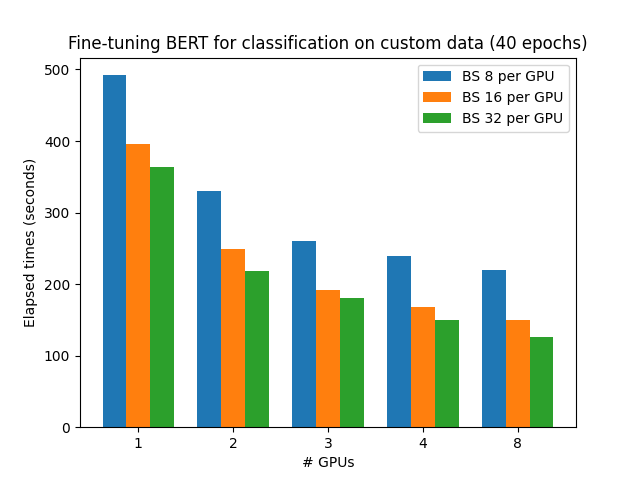
\includegraphics[width=0.7\columnwidth]{fig/benchmark_bybs_1.png}
    \caption{Wall clock time of fine-tuning BERT on various number of graphic cards on DGX}
    \label{fig:bert_benchmark}
\end{figure}


% \noindent\textbf{Subheading.} is a sample of how you can use a bold text without indentation. This
% technique can be handy if you want to stress the key topic that is going to be discussed in this
% paragraph. Example below.

% \noindent\textbf{Our goal.} The goal of this template is threefold. First, I want to make sure that
% everyone gets familiar with LaTeX, which is a very handy everyone should use when writing papers.

 
 

% \blfootnote{The repository URL: \url{https://github.com/calzonelover/Profiling-Transformer-Based-Model}}

\section{Background and Previous Works}

This section will walk through the concept of transfer learning that we are using in this work. Secondly, the explanation for the model architecture will be provided. Lastly, we briefly talk about the hardware that we use to benchmark in this work.

\subsection{Transfer Learning}

Transfer Learning is a method of machine learning. You can use the pre-trained model from the large general dataset to train your dataset or target tasks with a smaller dataset size, which is more efficient than training the model from scratch.~\cite{brownlee2017gentle}

\subsection{Transformer, BERT, RoBERTa, and GPT-2}

The Transformer is a model architecture of deep learning. It works with stacked self-attention and encoder/decoder stacks.~\cite{vaswani2017attention}

Bidirectional Encoder Representations (or BERT) from Transformers is sophisticated modified version of encoder part from transformer-based language model. It can be used as a pre-trained model from a large corpus to fine-tune with the specific dataset.~\cite{devlin2018bert} For RoBERTa, it is a transformer-based language model with an optimized method from the BERT model. RoBERTa is built on BERT but has different key hyperparameters, implementation, trained with dynamic masking, and removal of BERT's next sentence.~\cite{liu2019roberta}

GPT-2 is also a transformer-based language model with 1.5 billion parameters. It trained by large dataset from internet with 8 million web pages. Since it is a bloated model, it can learn with zero-shot setting.~\cite{radford2019better}

\begin{figure}[htbp]
  \centering
  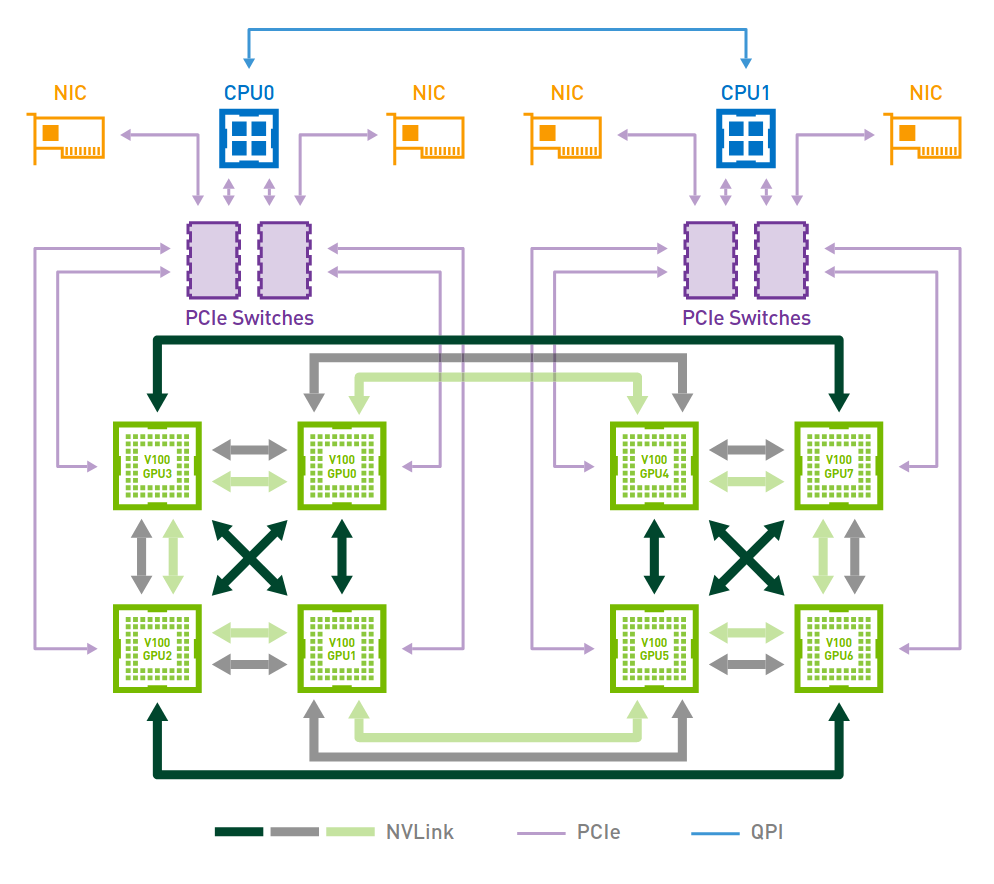
\includegraphics[width=0.6\linewidth]{fig/dgx-arch.png}
  \caption{Schematic view of DGX-1. Image taken from \cite{dgx-1}}
  \label{fig:dgx}
\end{figure}



\subsection{NVIDIA DGX-1}

The testing hardware is NVIDIA DGX-1. It consists of 8$\times$Tesla V100 GPUs, and each of them has 32 GB of attached memory. High level overview of this architecture is illustrated in Figure~\ref{fig:dgx}. The characteristic of these multi-GPUs devices is the NVLink. It is the inter-connection to reduce network latency in data sending across the devices. \cite{dgx-1}

%%%% This class file is first developed by Yoongu Kim for his PhD Thesis while at CMU and I would like to give all the credit to him. -- Rachata Ausavarungnirun

\LoadClass[11pt, oneside, letterpaper]{article}

%%%%%%%%%%%%%%%%%%%%%%%%%%%%%%%%%%%%%%%%%%%%%%%%%%%%%%%%%%%%%%%%%%%%%%%%%%%%%%%%
% Packages
%%%%%%%%%%%%%%%%%%%%%%%%%%%%%%%%%%%%%%%%%%%%%%%%%%%%%%%%%%%%%%%%%%%%%%%%%%%%%%%%

% margin
\RequirePackage{geometry}
\geometry{top=1.0in, bottom=1.0in, left=1.0in, right=1.0in}

% line spacing
\RequirePackage{setspace} % \setstretch, \singlespacing, \onehalfspacing, \doublespacing

% filler text
\RequirePackage[english]{babel}
\RequirePackage{blindtext} % \blindtext

% header
\RequirePackage{fancyhdr}

% title formatting
\RequirePackage{titling} % \thetitle, \thedate, \theauthor, \droptitle
\RequirePackage{titlesec}
\titlelabel{\thetitle.\hspace{0.4em}}
\titleformat*{\section}{\bf\fontsize{15pt}{15pt}\selectfont}
\titleformat*{\subsection}{\bf\fontsize{12pt}{12pt}\selectfont}
\titleformat*{\subsubsection}{\em\fontsize{12pt}{12pt}\selectfont}

% lists
\RequirePackage{enumitem} % \begin{itemize}, \begin{enumerate}
%\setlist{partopsep=0pt, topsep=0pt, itemsep=0pt, parsep=0pt}

% graphics
\RequirePackage{graphicx} % \includegraphics

% caption
\RequirePackage[labelsep=period, labelfont=bf]{caption}
\RequirePackage{subcaption}

% tables
\RequirePackage{booktabs}   % \toprule, \midrule, \cmidrule, \bottomrule
\RequirePackage{multirow}   % \multirow, \multicolumn
\RequirePackage{tabularx}   % \tabularx


% text
\RequirePackage{indentfirst}  % indent first paragraph
\RequirePackage[table]{xcolor}

% algorithm
\RequirePackage{algorithm}  % the floater wrapper for algorithmic
\RequirePackage[noend]{algpseudocode}
\RequirePackage{algorithmicx}

% math & units
\RequirePackage[text-rm]{siunitx}
\mathchardef\mhyphen="2D

% symbols
\RequirePackage{stmaryrd}

% fonts
\RequirePackage[scaled]{helvet}    % helvetica is larger than times
\newcommand{\hel}{\fontfamily{phv}\selectfont}

% table of contents
\RequirePackage[nottoc,numbib]{tocbibind}


%%%%%%%%%%%%%%%%%%%%%%%%%%%%%%%%%%%%%%%%%%%%%%%%%%%%%%%%%%%%%%%%%%%%%%%%%%%%%%%%
% Bibliography
%%%%%%%%%%%%%%%%%%%%%%%%%%%%%%%%%%%%%%%%%%%%%%%%%%%%%%%%%%%%%%%%%%%%%%%%%%%%%%%%
\bibliographystyle{abbrv}


%%%%%%%%%%%%%%%%%%%%%%%%%%%%%%%%%%%%%%%%%%%%%%%%%%%%%%%%%%%%%%%%%%%%%%%%%%%%%%%%
% Fonts
%%%%%%%%%%%%%%%%%%%%%%%%%%%%%%%%%%%%%%%%%%%%%%%%%%%%%%%%%%%%%%%%%%%%%%%%%%%%%%%%

%\RequirePackage{fontspec}
%\setmainfont[Ligatures=TeX]{Times New Roman}

%\RequirePackage{ebgaramond}
%\newfontfamily{\smallcaps}[RawFeature={+c2sc,+scmp}]{EB Garamond}
%\setromanfont[Numbers=OldStyle, Ligatures={Common}]{EB Garamond}
%\setsansfont[Scale=MatchLowercase, BoldFont={Lato Bold}]{Lato Regular}
%\setmonofont[Scale=MatchLowercase]{Source Code Pro}

\begin{table}[h!]
	\centering
	\begin{tabular}{lp{4.7in}}
		\toprule

		{\em Duration} & {\em Description} \\\midrule

		13 October 2021 & Submit Project Proposal  \\\midrule
%
		14 October - 14 December 2021 & Work on Profiling model \\\midrule

		15 December 2021 & Present Project \\\midrule

		17 December 2021 & Submit Project Report. \\ \bottomrule

	\end{tabular}
	\caption{Tentative timeline.}
	\label{tbl:timeline}
\end{table}



\section{Profiling Results} \label{sec:profiling}

We produce the profiling results from our source code, and we release our source code on GitHub.\footnote{https://github.com/calzonelover/Profiling-Transformer-Based-Model}

\subsection{RoBERTa}

\subsubsection{Configurations}
The configurations for RoBERTa model are as follows:
\begin{itemize}
    \item Batch size: 8
    \item GPU: 1, 2 and 4
    \item Model name: Wangchanberta (Thai RoBERTa model) \cite{wangchanberta2021}
    \item Dataset: Wongnai\_reviews (Text classification)
    \item Epoch: 1
\end{itemize}

\subsubsection{Results}
The simplest way to observe longest running interface could be done by aggregating each running interface. According to the Table~\ref{fig:bert:tg}, top 10 interfaces in single and double GPUs are all matrix multiplicative operations. On the other hand, most of  top 10 interfaces in 4 GPUs are collective communication in the GPU devices which are reduce and broadcast interfaces to transfer the data around the system. This is the first obvious clue to perform further study about how they spend the time on each group of interface to determine the problem from low level aspect.

\begin{figure}[htbp]
    \centering
    \begin{subfigure}{.5\textwidth}
        \centering
        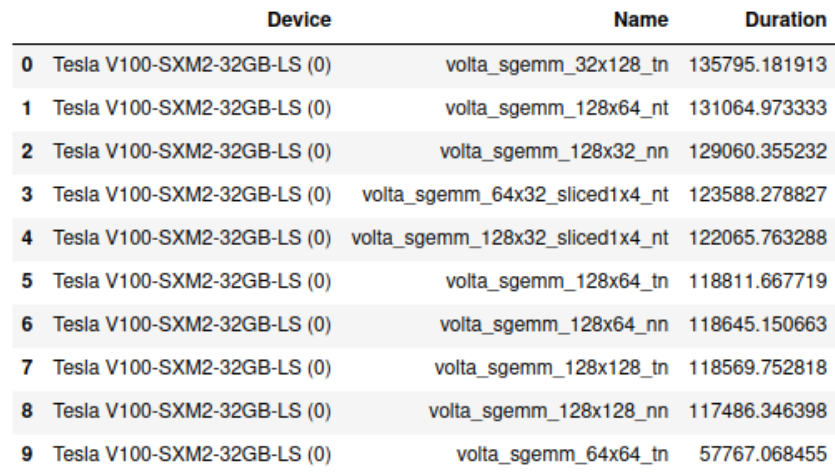
\includegraphics[width=\linewidth]{fig/bert/bert_t1.png}
        \caption{1 GPUs}
        \label{fig:bert:timegroup}
    \end{subfigure}%
    \begin{subfigure}{.5\textwidth}
        \centering
        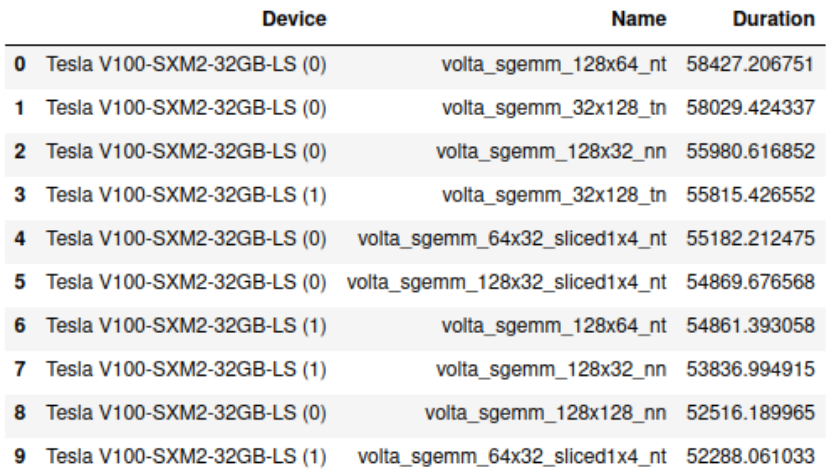
\includegraphics[width=\linewidth]{fig/bert/bert_t2.png}
        \caption{2 GPUs}
        \label{fig:bert:timegroup_frac}
    \end{subfigure}
    \begin{subfigure}{.6\textwidth}
        \centering
        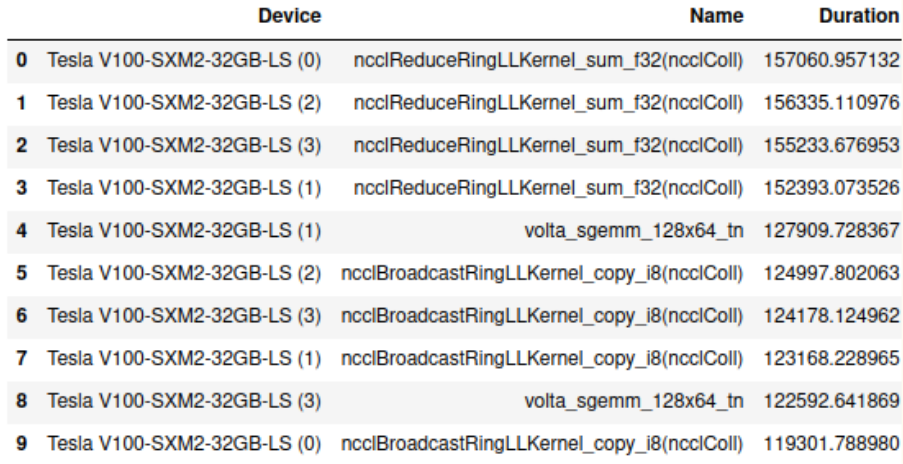
\includegraphics[width=\linewidth]{fig/bert/bert_t4.png}
        \caption{4 GPUs}
        \label{fig:bert:timegroup_frac}
    \end{subfigure}    
    \caption{Top 10 longest running interfaces}
\label{fig:bert:tg}
\end{figure}


The big picture of the problem can be seen by visualizing the aggregated running time of each operation group as in Figure~\ref{fig:bert:group_runtime}. It can bee seen that increasing the number of GPU will increase the spending time in memory management operations which is what we suspect in the first place. Moreover, running this model on four GPUs does induce a lot of collective communication across the devices to send the data back and forth. The memory management operation is more than 30\% of the overall running time. This is very critical for the scalability. It also implicitly means that the speed up factor after adding more than 4 GPUs might not significant anymore. Hence, we probably under-utilize the resource when training BERT model with more than four GPUs.


\begin{figure}[htbp]
    \centering
    \begin{subfigure}{.5\textwidth}
        \centering
        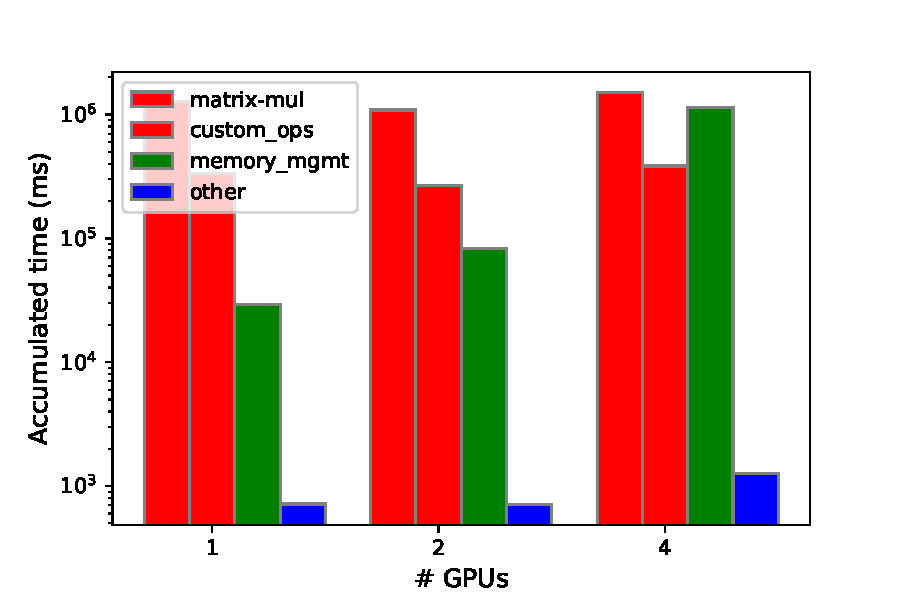
\includegraphics[width=\linewidth]{fig/bert/timegroup.pdf}
        \caption{Real spending time}
        \label{fig:bert:timegroup}
    \end{subfigure}%
    \begin{subfigure}{.5\textwidth}
        \centering
        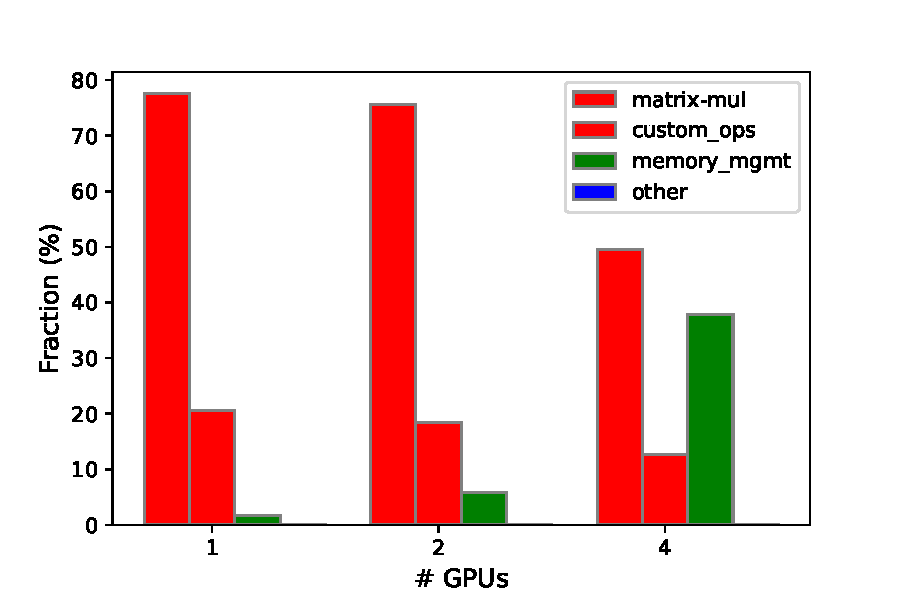
\includegraphics[width=\linewidth]{fig/bert/timegroup_frac.pdf}
        \caption{Fraction of time}
        \label{fig:bert:timegroup_frac}
    \end{subfigure}
    \caption{Spending time of multiple group of operations}
\label{fig:bert:group_runtime}
\end{figure}

\begin{figure}[htbp]
    \centering
    \begin{subfigure}{.5\textwidth}
      \centering
      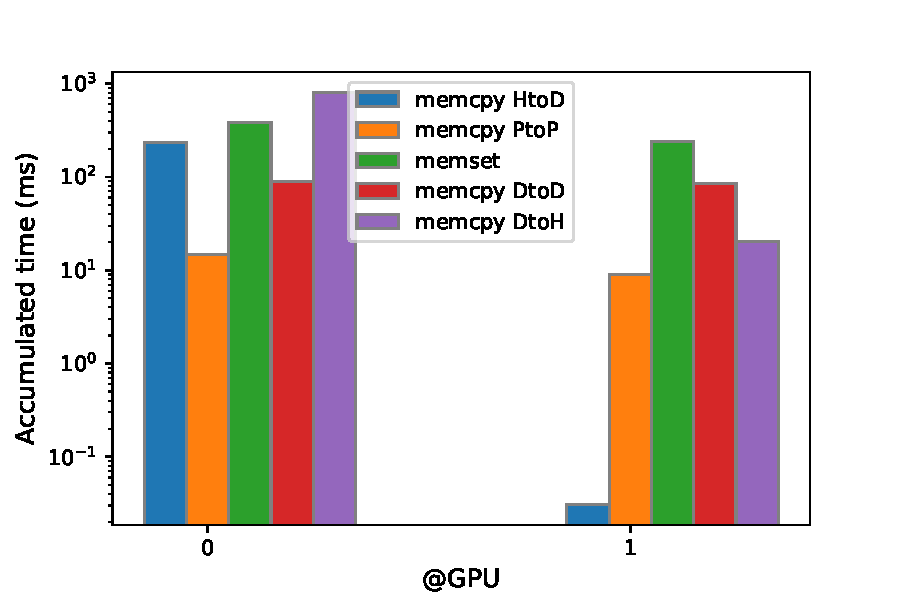
\includegraphics[width=\linewidth]{fig/bert/mem_2gpus.pdf}
      \caption{2 GPUs}
    \end{subfigure}%
    \begin{subfigure}{.5\textwidth}
      \centering
      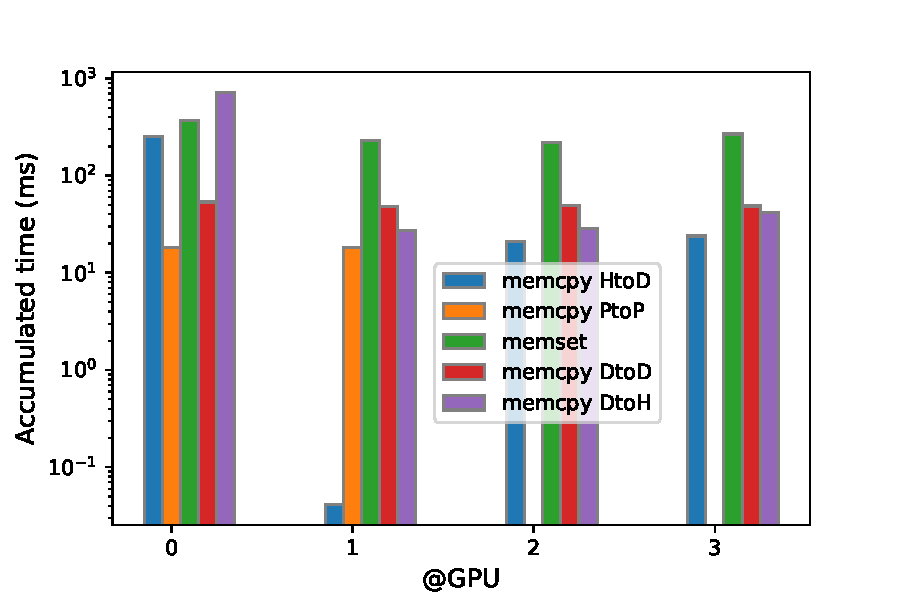
\includegraphics[width=\linewidth]{fig/bert/mem_4gpus.pdf}
      \caption{4 GPUs}
    \end{subfigure}
    \caption{Aggregated runtime of the built-in memory management operations}
\label{fig:bert:mem_mgnt}
\end{figure}


Since the memory management operations is likely to be the main factor of the poor speed up factor. Digging into their sub-group operations especially the built-in memory allocation and transfer function could bring us closer to the root cause of the communication overhead. Figure~\ref{fig:bert:mem_mgnt} demonstrates the aggregated run-time in each built-in operations. There is an asymmetric behaviour in the memory transfer of host-to-device and device-to-host where the second GPU barely see host-to-device operation for both cases. Moreover, the first GPU tends to volunteer to do this task. Device-to-host operation is more balance with a little asymmetry in the first GPU that they are significantly does consume more run-time by one order of magnitude.


\subsection{GPT-2}

\subsubsection{Configurations}

The configurations for GPT-2 model are as follows:

\begin{itemize}
    \item Batch size: 4
    \item GPU: 1, 2 and 4
    \item Model name: DistilGPT2 (the smallest version of GPT2)
    \item Dataset: Yelp Dataset (Text Classification)
    \item Epoch: 1
\end{itemize}

\subsubsection{Results}

Similar to BERT model, the top 10 most longest running interfaces in GPT-2 does have the same problem with communication overhead. Considering the Figure~\ref{fig:gpt2:tg}, The collective communication operators even appears when we train on a couple of GPUs and it getting worse when the number of GPUs reaching to four.

\begin{figure}[htbp]
    \centering
    \begin{subfigure}{.5\textwidth}
        \centering
        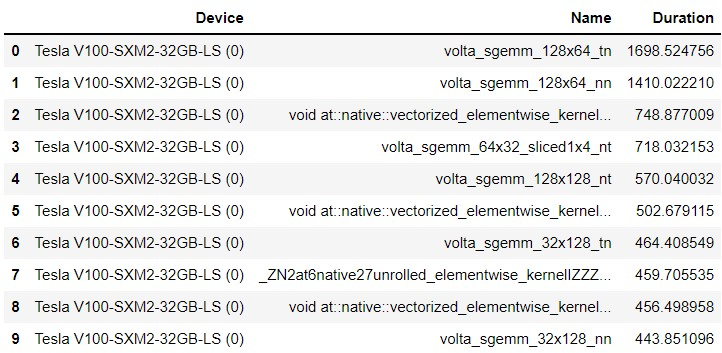
\includegraphics[width=\linewidth]{fig/gpt2/gpt_t1.jpg}
        \caption{1 GPUs}
        \label{fig:gpt2:timegroup}
    \end{subfigure}%
    \begin{subfigure}{.5\textwidth}
        \centering
        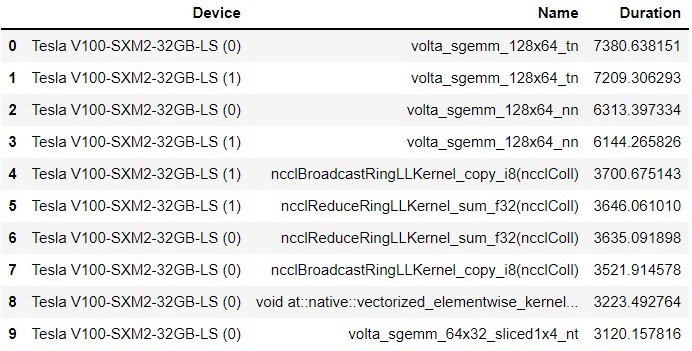
\includegraphics[width=\linewidth]{fig/gpt2/gpt_t2.jpg}
        \caption{2 GPUs}
        \label{fig:gpt2:timegroup_frac}
    \end{subfigure}
    \begin{subfigure}{.6\textwidth}
        \centering
        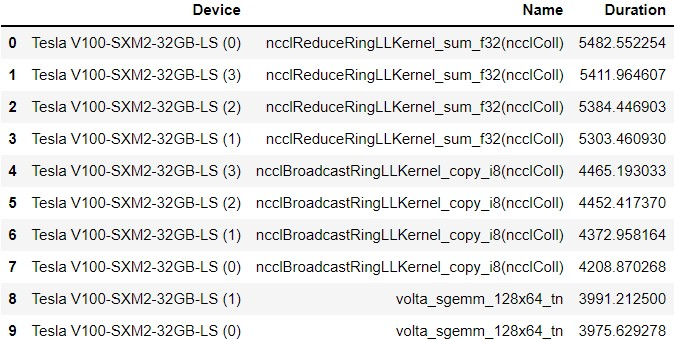
\includegraphics[width=\linewidth]{fig/gpt2/gpt_t4.jpg}
        \caption{4 GPUs}
        \label{fig:gpt2:timegroup_frac}
    \end{subfigure}    
    \caption{Top 10 longest running interfaces}
\label{fig:gpt2:tg}
\end{figure}

% For The big picture of the problem, It is like the results of the BERT model from visualizing the aggregated running time of each operation group as in Figure~\ref{fig:gpt2:group_runtime}
The trivial observations is illustrated in Figure~\ref{fig:gpt2:group_runtime}, it does have the same problem of data transfer where running on GPUs does spending more than one third of their time. Regarding to the Figure~\ref{fig:gpt2:mem}, the asymmetric in the host-to-device operation among running devices is more severe. The rest of them barely do host-to-device task. Surprisingly, memset operation is also unbalanced in four GPUs running which is not similar to a two GPUs and all benchmark in BERT.

\begin{figure}[htbp]
    \centering
    \begin{subfigure}{.5\textwidth}
        \centering
        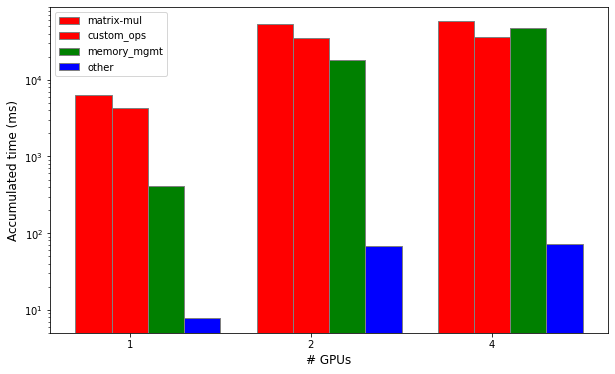
\includegraphics[width=\linewidth]{fig/gpt2/timegroup.png}
        \caption{Real spending time}
        \label{fig:gpt2:timegroup}
    \end{subfigure}%
    \begin{subfigure}{.5\textwidth}
        \centering
        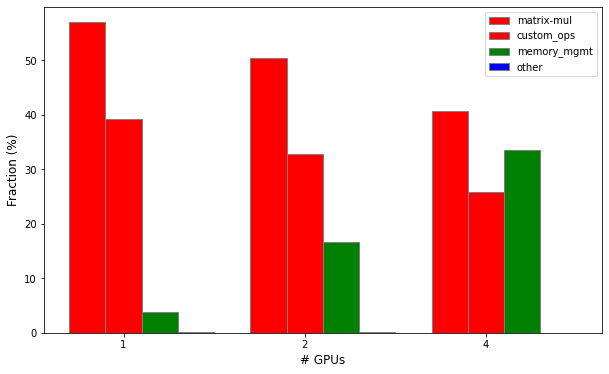
\includegraphics[width=\linewidth]{fig/gpt2/timegroup_frac.png}
        \caption{Fraction of time}
        \label{fig:gpt2:timegroup_frac}
    \end{subfigure}
    \caption{Spending time of multiple group of operations}
\label{fig:gpt2:group_runtime}
\end{figure}

\begin{figure}[htbp]
    \centering
    \begin{subfigure}{.5\textwidth}
      \centering
      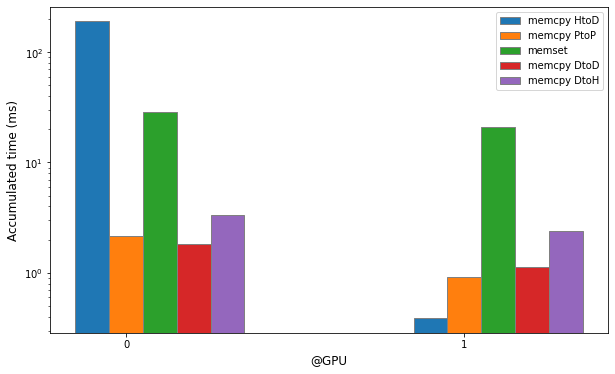
\includegraphics[width=\linewidth]{fig/gpt2/men_2gpu.png}
      \caption{2 GPUs}
      \label{fig:sub1}
    \end{subfigure}%
    \begin{subfigure}{.5\textwidth}
      \centering
      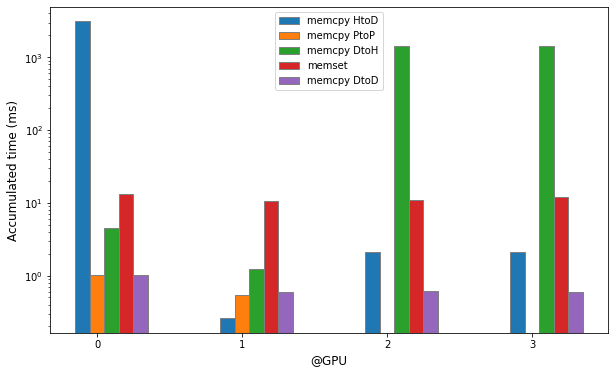
\includegraphics[width=\linewidth]{fig/gpt2/men_4gpu.png}
      \caption{4 GPUs}
      \label{fig:sub2}
    \end{subfigure}
    \caption{Aggregated runtime of the built-in memory management operations}
\label{fig:gpt2:mem}
\end{figure}

% \textcolor{red}{Discuss the result with figures}
\section{Conclusion} \label{sec:conclusion}

We investigate the kernel/interface calling from the training process. The results show that as the number of GPUs increases, the communication overhead is also introduced to the system. It means that the horizontal scaling for GPU training is highly non-linear. In addition, we also found an asymmetry in spending time on memory management regarding the multi-GPUs regime.


%%%%%%%%%%%%%%%%%%%%%%%%%%%%%%%%%%%%%%%%%%%%%%%%%%%%%%%%%%%%%%%%%%%%%%%%%%%%%%%%
% bibliography
%%%%%%%%%%%%%%%%%%%%%%%%%%%%%%%%%%%%%%%%%%%%%%%%%%%%%%%%%%%%%%%%%%%%%%%%%%%%%%%%
%\clearpage
\small
\singlespacing
\bibliography{references}
\newpage
\section{Appendix} \label{sec:appendix}

\textbf{Hardware}
\begin{itemize}
    \item Nvidia DGX-1
    \item GPU: Tesla V100 x 8
    \item CPU: Intel(R) Xeon(R) CPU E5-2698 v4 @ 2.20GHz
    \item RAM: 503 GB
\end{itemize}

\textbf{Software}
\begin{itemize}
    \item nvprof	10.2.89
    \item python	3.6
    \item CUDA	NVIDIA-SMI 450.119.04  
    \item Driver Version: 450.119.04 
    \item CUDA Version: 11.0
    \item Running on (Docker) Container
    \item Docker image: nvcr.io/nvidia/pytorch:19.11-py3
\end{itemize}


% \subsection{Source Code}

% \subsubsection{BERT}
% \label{src:bert}
% \lstinputlisting[language=Python]{src/bert.py}

% \subsubsection{GPT-2}
% \label{src:gpt}
% \lstinputlisting[language=Python]{src/gpt.py}

\end{document}

